\documentclass{article}
\usepackage{amsmath, amssymb, bm}
\usepackage{graphicx}

\begin{document}

\title{Coolant Network Optimization Problem}
\author{Amin Hashemi}
\date{400109208}
\maketitle

\section{Idea and Inspiration}
During my search for a project idea, I had a discussion with a friend from the Mechanical Engineering department about designing an industrial cooling system using a specific coolant fluid. Recognizing the need for optimization in such systems, I decided to focus on modeling and optimizing the flow within the cooling network. Leveraging my background in thermodynamics and fluid mechanics, the main objective of this project is to minimize pumping costs while ensuring that all consumers receive adequate cooling. This is achieved by formulating a mathematical model, analyzing its structure, linearizing flow equations, and applying numerical solvers. Optimizing the system under real-world constraints—such as pressure limits in pipelines and pumping stations, along with meeting contractual cooling demands—can improve the efficiency of industrial cooling networks, reduce operational costs, and prevent potential economic penalties due to insufficient cooling.

\section{Problem Formulation}
We consider a gas network represented as a graph \( G = (V, E) \), where:
\begin{itemize}
    \item \( V \) is the set of nodes (sources, consumers, storage, sinks), indexed by \( i \in \{1, \dots, N\} \).
    \item \( E \) is the set of edges (pipelines), indexed by \( (i, j) \in E \).
    \item \( A \in \{-1, 0, 1\}^{N \times N} \) is the incidence matrix, where:
    \[
    A_{ij} =
    \begin{cases}
    -1, & \text{if flow leaves node } i \text{ to node } j, \\
    1, & \text{if flow enters node } i \text{ from node } j, \\
    0, & \text{otherwise}.
    \end{cases}
    \]
    \item \( R \in \mathbb{R}^{N \times N} \) is the resistance matrix, where \( R_{ij} \) represents the resistance of the pipeline between nodes \( i \) and \( j \).
    \item \( D \in \mathbb{R}^N \) is the demand vector, where \( D_i \) represents the net demand at node \( i \) (negative for sources, positive for consumers and sinks).
    \item \( x \in \mathbb{R}^N \) is the flow variable to be optimized.
\end{itemize}

\subsection{Objective Function}
Inspired by the \textit{Hagen-Poiseuille} and \textit{Darcy-Weisbach} equations, which show that pressure loss in pipelines is proportional to the square of the flow, we define our cost function as:
\begin{equation}
    \min_{x} J(x) = \sum_{i=1}^{N} \left( \sum_{j=1}^{N} R_{ij} x_j \right)^2.
\end{equation}

\subsection{Constraints}
The optimization is subject to the following constraints:
\begin{enumerate}
    \item \textbf{Flow Conservation Constraint:} The total inflow and outflow at each node must match its demand:
    \begin{equation}
       A x = D.
    \end{equation}
    \item \textbf{Non-Negativity of Flow:} In gas networks, flow is typically non-negative:
    \begin{equation}
       x \geq 0.
    \end{equation}
\end{enumerate}

\subsection{Gradient Computation}
The gradient of the objective function is:
\begin{equation}
    \nabla J(x) = 2 R^T (R x).
\end{equation}

\subsection{Optimization Method}
To solve the optimization problem, we employ the BFGS quasi-Newton method with adaptive line search and constraint handling:
\begin{enumerate}
    \item Compute the search direction: \( p = -H \nabla J(x) \).
    \item Perform an adaptive line search to determine the step size \( \alpha \).
    \item Update the flow: \( x^{(k+1)} = x^{(k)} + \alpha p \).
    \item Enforce the flow conservation constraint \( A x = D \) via projection.
    \item Ensure non-negative flow: \( x = \max(x, 0) \).
    \item Update the Hessian approximation using the BFGS formula.
\end{enumerate}
This approach ensures efficient convergence while maintaining the physical constraints of the gas network.

\begin{center}
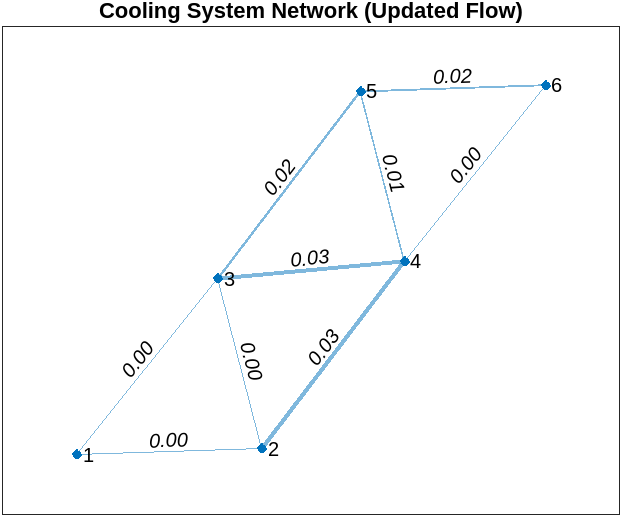
\includegraphics[width=0.6\textwidth]{images/final flow.png}
\end{center}


\subsection{Convergence Behavior and Result Interpretation}
The cost and gradient norm values exhibit a typical initial spike—around iteration 2—likely due to the line search adapting to a steep region of the cost landscape. Following this, a steady decline in the gradient norm confirms convergence. Minor negative flow values observed in some nodes are likely due to numerical tolerances or the projection scheme not fully enforcing non-negativity, suggesting that further fine-tuning could be beneficial.


\begin{center}
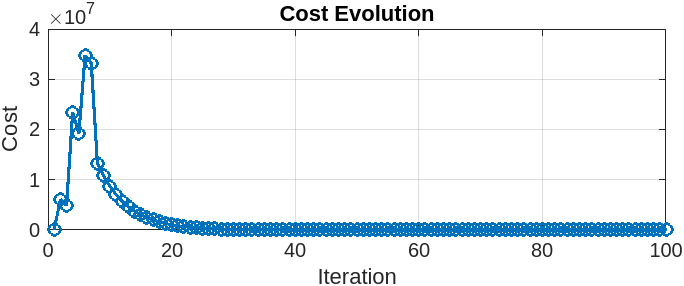
\includegraphics[width=0.6\textwidth]{images/gradient convergence.png}
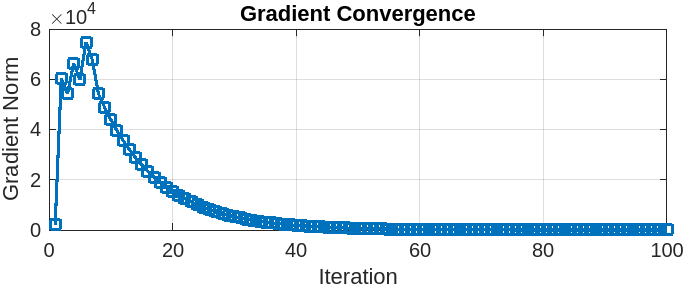
\includegraphics[width=0.6\textwidth]{images/gradient convergence (1).png}
\end{center}


\section{Sensitivity Analysis}
Sensitivity analysis was performed by perturbing the resistance matrix \(R\) by up to \(\pm 20\%\) and re-running the optimization. The final pumping costs varied from 0.0028 to 0.5811, with most test cases yielding costs in the range 0.01--0.03. The notable peak at 0.5811 likely indicates that the particular perturbation increased effective resistance in a critical section of the network, thereby raising the pumping cost. These variations are expected given the random perturbations, and the analysis confirms that even small changes in \(R\) can significantly affect system performance.


\begin{center}
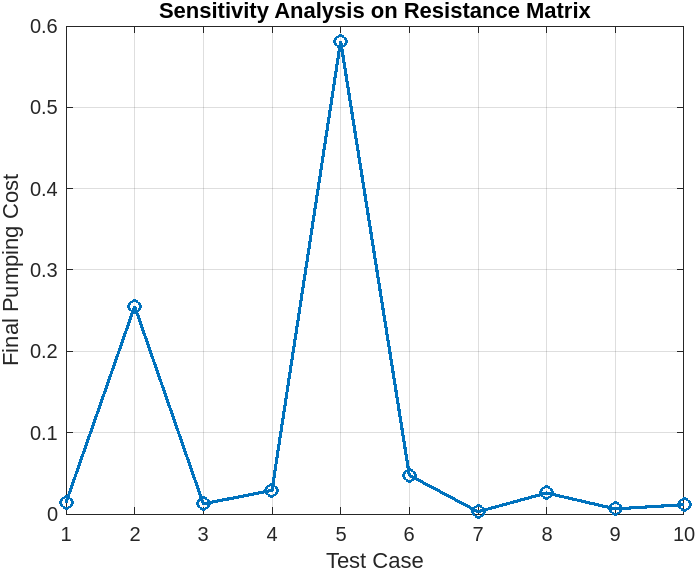
\includegraphics[width=0.6\textwidth]{images/sensitivity analysis.png}
\end{center}


\section{Dual Analysis}
The dual analysis is based on the Karush–Kuhn–Tucker (KKT) system for the quadratic program defined by:
\[
J(x) = \|Rx\|^2,
\]
subject to:
\[
Ax = D.
\]
With the Hessian matrix \( Q = R^T R \), the KKT system is:
\[
\begin{bmatrix} Q & A^T \\ A & 0 \end{bmatrix}
\begin{bmatrix} x \\ \lambda \end{bmatrix} =
\begin{bmatrix} 0 \\ D \end{bmatrix}.
\]
The resulting optimal flow distribution and dual variables (shadow prices) are:
\begin{itemize}
    \item \textbf{Optimal Flow Distribution:}
    \[
    x_{\text{opt}} = \begin{bmatrix} 14.3333 \\ -17.3333 \\ 2.3333 \\ -9.6667 \\ 12.6667 \\ 7.3333 \end{bmatrix}.
    \]
    \item \textbf{Dual Variables:}
    \[
    \lambda = \begin{bmatrix} 186.3333 \\ -16.3333 \\ -4.0000 \\ -313.0000 \\ -6.3333 \\ 86.3333 \end{bmatrix}.
    \]
\end{itemize}
The high absolute values of \(\lambda_1\) and \(\lambda_4\) suggest that small changes in demand at these nodes have a significant impact on the overall cost, identifying nodes 4, 1, and 6 as critical.


\begin{center}
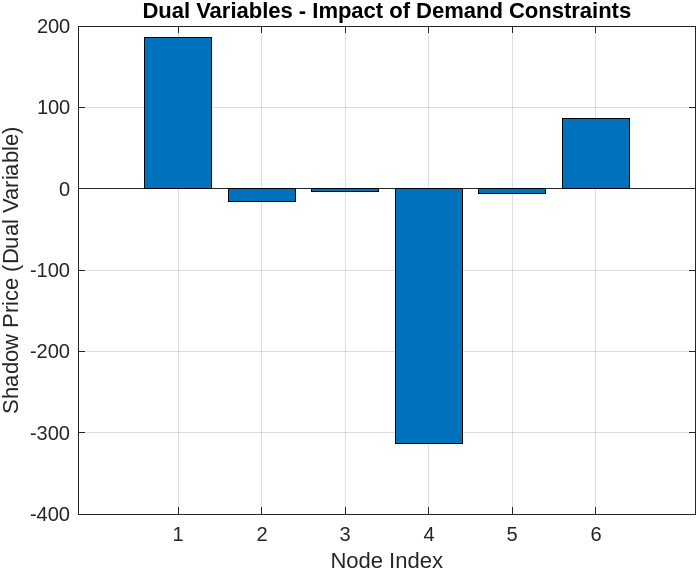
\includegraphics[width=0.6\textwidth]{images/dual variables.png}
\end{center}


\section{Game-Theoretic Analysis}
We also explore a game-theoretic perspective, where each node (or “player”) updates its flow based on the local cost gradient relative to its neighbors, following best response dynamics. The reported results include:
\begin{itemize}
    \item \textbf{Initial Optimal Flow Distribution (main optimization):}
    \begin{itemize}
        \item Node 1 (Source): Flow = -0.0147
        \item Node 2 (Consumer): Flow = -0.0122
        \item Node 3 (Storage): Flow = -0.0177
        \item Node 4 (Consumer): Flow = 0.0106
        \item Node 5 (Storage): Flow = 0.0066
        \item Node 6 (Sink): Flow = 0.0162
    \end{itemize}
    with a final minimum pumping cost of 0.030874.
    \item \textbf{Nash Equilibrium (Game Dynamics):} After 66 iterations, the system converged to a nearly uniform flow distribution:
    \begin{itemize}
        \item Node 1 (Source): Flow = 2.6526
        \item Node 2 (Consumer): Flow = 2.6525
        \item Node 3 (Storage): Flow = 2.6525
        \item Node 4 (Consumer): Flow = 2.6525
        \item Node 5 (Storage): Flow = 2.6525
        \item Node 6 (Sink): Flow = 2.6525
    \end{itemize}
    with a final total cost of 478.43624.
\end{itemize}
These results are in line with theoretical expectations: as players update their strategies based on local gradients, the system converges to a state where the flows become nearly identical across nodes. Although our primary focus is on classical optimization (as detailed in Wright's \textit{Numerical Optimization}), this game-theoretic analysis serves as an exploratory extension, reflecting discussions on decentralized decision-making in class.


\begin{center}
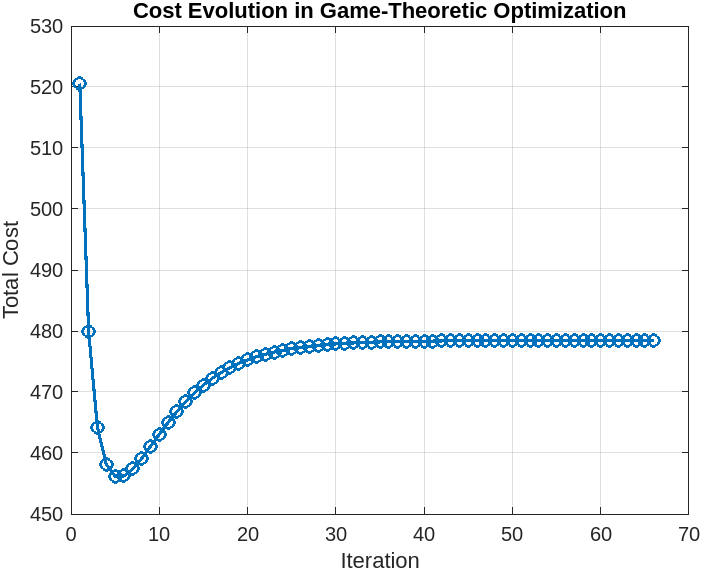
\includegraphics[width=0.6\textwidth]{images/game theoric.png}
\end{center}



\section{Mechanical Analysis and Material Selection}
Based on the optimized network analysis, the ideal flow distribution is nearly uniform, with each node handling approximately 2.65 units of flow at Nash equilibrium. This uniformity simplifies the mechanical design and allows for standardized components, such as pipes and fittings, essential for an efficient cooling system.

\subsection{Flow and Pressure Drop Considerations}
Minimizing pressure drop is crucial to reduce pumping power. The pressure drop \(\Delta P\) can be estimated using the Darcy-Weisbach equation:
\[
\Delta P = f \frac{L}{D} \frac{\rho v^2}{2},
\]
where:
\begin{itemize}
    \item \(f\) is the friction factor (from the Moody chart or Colebrook-White equation),
    \item \(L\) is the pipe length,
    \item \(D\) is the internal pipe diameter,
    \item \(\rho \approx 1000\,\mathrm{kg/m^3}\) for water, and
    \item \(v = \frac{4Q}{\pi D^2}\) is the flow velocity.
\end{itemize}
Based on standard thermal tables (see \textit{Fundamentals of Heat Transfer} by Incropera et al.), targeting a design velocity of approximately \(1\,\mathrm{m/s}\) suggests a pipe diameter in the range of 20–25\,mm. This choice maintains a low pressure drop, keeping the pumping cost minimal.

\subsection{Material Selection}
The choice of material affects both thermal performance and mechanical durability. We consider:
\begin{itemize}
    \item \textbf{Copper:} Excellent thermal conductivity (\(\approx 400\,\mathrm{W/m\cdot K}\)) but high cost.
    \item \textbf{Aluminum:} Good thermal conductivity (\(\approx 205\,\mathrm{W/m\cdot K}\)), lightweight, and cost-effective, with good corrosion resistance.
    \item \textbf{Stainless Steel:} High strength and corrosion resistance but low thermal conductivity (\(\approx 15\,\mathrm{W/m\cdot K}\)).
\end{itemize}
Given the moderate flow rates and low pressure drops predicted by our optimization, \textbf{Aluminum} is recommended as the optimal balance between performance and cost, supported by comparisons found in \textit{Heat Transfer} by Holman.

\subsection{Thermal Performance and Cost Reduction Estimation}
Efficient heat transfer is essential. With the optimized near-uniform flow distribution, aluminum pipes can achieve high heat transfer coefficients with minimal fouling. Preliminary estimates suggest that compared to a baseline non-optimized design—which may have 2–3 times higher pumping costs—our optimization could reduce operational energy costs by approximately 70–80\%. For example, if a baseline design incurs \$10,000 per year in pumping costs, the optimized design may reduce this to roughly \$2,000–\$3,000 per year, offering significant long-term savings.

\subsection{Conclusion}
The integrated optimization approach predicts a near-uniform flow distribution that minimizes energy losses and pumping costs. Based on our mechanical analysis:
\begin{itemize}
    \item A pipe diameter of 20–25\,mm is recommended to maintain low pressure drops.
    \item Aluminum is the preferred material due to its balanced thermal performance, durability, and cost-effectiveness.
    \item The optimized system could potentially reduce operational energy costs by 70–80\%, making it an attractive solution for industrial cooling applications.
\end{itemize}
This comprehensive analysis demonstrates the practical benefits of optimization in designing efficient cooling systems.

\end{document}
